\documentclass[paper=letter,11pt]{scrartcl}

\KOMAoptions{headinclude=true, footinclude=false}
\KOMAoptions{DIV=14, BCOR=5mm}
\KOMAoptions{numbers=noendperiod}
\KOMAoptions{parskip=half}
\addtokomafont{disposition}{\rmfamily}
\addtokomafont{part}{\LARGE}
\addtokomafont{descriptionlabel}{\rmfamily}
%\setkomafont{pageheadfoot}{\normalsize\sffamily}
\setkomafont{pagehead}{\normalsize\rmfamily}
%\setkomafont{publishers}{\normalsize\rmfamily}
\setkomafont{caption}{\normalfont\small}
\setcapindent{0pt}
\deffootnote[1em]{1em}{1em}{\textsuperscript{\thefootnotemark}\ }


\usepackage{amsmath}
\usepackage[varg]{txfonts}
\usepackage[T1]{fontenc}
\usepackage{graphicx}
\usepackage{xcolor}
\usepackage[american]{babel}
% hyperref is needed in many places, so include it here
\usepackage{hyperref}

\usepackage{xspace}
\usepackage{multirow}
\usepackage{float}


\usepackage{braket}
\usepackage{bbm}
\usepackage{relsize}
\usepackage{tcolorbox}


\def\x{\ensuremath{x}}
\def\xp{\ensuremath{x'}}
\def\t{\ensuremath{t}}
\def\tp{\ensuremath{t'}}
\def\v{\ensuremath{v}}
%\def\nus{$\nu$s}

%\def\ketY{\ensuremath{\ket {\Psi}}}
%\def\iGeV{\ensuremath{\textrm{GeV}^{-1}}}
%%\def\mp{\ensuremath{m_{\textrm{proton}}}}
%\def\rp{\ensuremath{r_{\textrm{proton}}}}
%\def\me{\ensuremath{m_{\textrm{electron}}}}
%\def\aG{\ensuremath{\alpha_G}}
%\def\rAtom{\ensuremath{r_{\textrm{atom}}}}
%\def\rNucl{\ensuremath{r_{\textrm{nucleus}}}}
%\def\GN{\ensuremath{\textrm{G}_\textrm{N}}}
%\def\ketX{\ensuremath{\ket{\vec{x}}}}
%\def\ve{\ensuremath{\vec{\epsilon}}}
%
%
%\def\ABCDMatrix{\ensuremath{\begin{pmatrix} A &  B  \\ C  & D \end{pmatrix}}}
%\def\xyprime{\ensuremath{\begin{pmatrix} x' \\ y' \end{pmatrix}}}
%\def\xyprimeT{\ensuremath{\begin{pmatrix} x' &  y' \end{pmatrix}}}
%\def\xy{\ensuremath{\begin{pmatrix} x \\ y \end{pmatrix}}}
%\def\xyT{\ensuremath{\begin{pmatrix} x & y \end{pmatrix}}}
%
%\def\IMatrix{\ensuremath{\begin{pmatrix} 0 &  1  \\ -1  & 0 \end{pmatrix}}}
%\def\IBoostMatrix{\ensuremath{\begin{pmatrix} 0 &  1  \\ 1  & 0 \end{pmatrix}}}
%\def\JThree{\ensuremath{\begin{pmatrix}    0 & -i & 0  \\ i & 0  & 0 \\ 0 & 0 & 0 \end{pmatrix}}} 
%\def\JTwo{\ensuremath{\begin{bmatrix}    0 & 0 & -i  \\ 0 & 0  & 0 \\ i & 0 & 0 \end{bmatrix}}}
%\def\JOne{\ensuremath{\begin{bmatrix}    0 & 0 & 0  \\ 0 & 0  & -i \\ 0 & i & 0 \end{bmatrix}}}
%\def\etamn{\ensuremath{\eta_{\mu\nu}}}
%\def\Lmn{\ensuremath{\Lambda^\mu_\nu}}
%\def\dmn{\ensuremath{\delta^\mu_\nu}}
%\def\wmn{\ensuremath{\omega^\mu_\nu}}
%\def\be{\begin{equation*}}
%\def\ee{\end{equation*}}
%\def\bea{\begin{eqnarray*}}
%\def\eea{\end{eqnarray*}}
%\def\bi{\begin{itemize}}
%\def\ei{\end{itemize}}
%\def\fmn{\ensuremath{F_{\mu\nu}}}
%\def\fMN{\ensuremath{F^{\mu\nu}}}
%\def\bc{\begin{center}}
%\def\ec{\end{center}}
%\def\nus{$\nu$s}

\def\adagger{\ensuremath{a_{p\sigma}^\dagger}}
\def\lineacross{\noindent\rule{\textwidth}{1pt}}

\newcommand{\multiline}[1] {
\begin{tabular} {|l}
#1
\end{tabular}
}

\newcommand{\multilineNoLine}[1] {
\begin{tabular} {l}
#1
\end{tabular}
}



\newcommand{\lineTwo}[2] {
\begin{tabular} {|l}
#1 \\
#2
\end{tabular}
}

\newcommand{\rmt}[1] {
\textrm{#1}
}


%
% Units
%
\def\m{\ensuremath{\rmt{m}}}
\def\GeV{\ensuremath{\rmt{GeV}}}
\def\pt{\ensuremath{p_\rmt{T}}}


\def\parity{\ensuremath{\mathcal{P}}}

\usepackage{cancel}
\usepackage{ mathrsfs }
\def\bigL{\ensuremath{\mathscr{L}}}

\usepackage{ dsfont }

\def\nus{$\nu$s}
\def\nue{\ensuremath{\nu_e}}
\def\numu{\ensuremath{\nu_\mu}}
\def\nutau{\ensuremath{\nu_\tau}}
\def\nualpha{\ensuremath{\nu_\alpha}}
\def\nuone{\ensuremath{\nu_1}}
\def\nutwo{\ensuremath{\nu_2}}
\def\nuthree{\ensuremath{\nu_3}}


\usepackage{fancyhdr}
\fancyhf{}



\lhead{\Large 33-211} % \hfill Introduction to Particle Physics \hfill Spring 2022}
\chead{\Large Physics 3 : Modern Essentials} % \hfill Spring 2022}
\rhead{\Large Spring 2023} % \hfill Introduction to Particle Physics \hfill Spring 2022}
\begin{document}
\thispagestyle{fancy}





%\begin{tabular}{c}
%{\large 33-444 \hfill Intro To Particle \hfill Spring 2019\\}
%\hline 
%\end{tabular}

\begin{center}
{\huge \textbf{Final Exam}}
\large

\end{center}

{\large


\textbf{1) Chased by a comet }\hfill \textit{(3 points)}\\
A comet is chasing a spaceship.
Let $\beta$, P and E be the speed, momentum, and energy of the comet as seen by the astronaut when it hits the spaceship. 
In what way would the increasing the spaceship's speed alter the astronaut's perceived values of $\beta$, P and E?
\begin{itemize}
\item[a)] $\beta$, P and E will all be constant not change at all.
\item[b)] $\beta$, P and E will all decrease.
\item[c)] $\beta$, P will get smaller, E will not change.
\item[d)] $\beta$, E will get smaller, P will not change.
\item[e)] P and E will get smaller, $\beta$ will not change.
\end{itemize}

\vfill

\textbf{2) Chased by a photon }\hfill \textit{(3 points)}\\
A photon is chasing a spaceship.
Let $\beta$, P and E be the speed, momentum, and energy of the photon as seen by the astronaut when it hits the spaceship. 
In what way would the increasing the spaceship's speed alter the astronaut's perceived values of $\beta$, P and E?
\begin{itemize}
\item[a)] $\beta$, P and E will all be constant not change at all.
\item[b)] $\beta$, P and E will all decrease.
\item[c)] $\beta$, P will get smaller, E will not change.
\item[d)] $\beta$, E will get smaller, P will not change.
\item[e)] P and E will get smaller, $\beta$ will not change.
\end{itemize}

\vfill

\textbf{3) Invariants }\hfill \textit{(8 points)}\\
Which of the following are invariant (ie: agreed on by all inertial observers)?
\begin{itemize}
\item[a)] time ordering of time-like separated events
\item[c)] component of the velocity of a projectile parallel to relative direction of motion
\item[b)] component of the velocity of a projectile perpendicular to relative direction of motion
\item[c)] time between events
\item[d)] distance between events
\item[e)] total particle speed when beta < 1
\item[f)] total particle speed when beta = 1
\item[g)] proper time along a world line
\end{itemize}

\clearpage

\textbf{4) Proper Times}  \hfill \textit{(6 points)}\\
Consider three paths through space time: $A\rightarrow P \rightarrow B$, $A\rightarrow Q \rightarrow B$, and $A\rightarrow R \rightarrow B$.\\
Where the points are given by:

\begin{tabular}{clr}
  & (x[m],& ct[m])\\
  \hline
  A = & (0, & 0)\\
  P = & (0, & 5/3)\\
  Q = & (4/3, & 5/3)\\
  R = & (5/3, & 5/3)\\
  B = & (0,    & 10/3)\\
\end{tabular}

What are the proper times of each of the three paths?

\vfill

\textbf{5) Lorentz Transformations}  \hfill \textit{(4 points)}\\
Which of the following is/are valid Lorentz transform?
\begin{itemize}
\item[a)] $p_x' = p_x - (3/4) E$ \\ $E' = E - (3/4) p_x$ \\
\item[b)] $p_x' = (5/4)p_x - (3/4) E$ \\ $E' = (5/4)E - (3/4) p_x$ \\
\item[c)] $p_x' = (5/4)p_x - (3/5) E$ \\ $E' = (3/5)E - (5/4) p_x$ \\
\item[d)] $p_x' = (3/4)p_x - (5/4) E$ \\ $E' = (5/4)E - (3/4) p_x$ \\
\item[d)] None of the above.
\end{itemize}

\clearpage


\textbf{6) Causality}  \hfill \textit{(10 points)}\\
You are located at the origin of the S frame: (x,t)=(0,0).
Your friend is located at the origin of the S` which is moving to the right at $\beta = 0.99$ wrt the S frame in the usual way with origins coinciding at (0,0).
Consider the following space-time events (coordinates in S):\\

\begin{tabular}{clr}
  & (x,& t)\\
  \hline
  A = & (0   , & 2)\\
  B = & (2.01, & 2)\\
  C = & (1.99, & 2)\\
  D = & (2,    & 0)\\
  E = & (0,    & -2)\\
  F = & (2,    & -1.99)\\
  G = & (2,    & -2.01)\\
\end{tabular}

\vspace{0.1in}

a) Which events can you causally effect ?\\

b) Which events can your friend causally effect ?\\

c) Which events can casually effect you?\\

d) Which events can casually effected your friend?

\clearpage

%a) Argue with a space diagram that casualty (ie: time-ordering) is preserved 
%is causes propogate at beta < 0. 
%
%\vspace{2in}
%b) Argue with a space diagram that casality (ie: time-ordering) is NOT preserved 
%if beta > 1
%\vspace{2in}


\textbf{7) Missiles in space}  \hfill \textit{(12 points)}\\
A Space-X starship rocket moves toward earth with speed 3/5c.
The crew shoots a missile sideways to this direction with speed 4/5c.
What is the velocity of the missile (magnitude and angle) relative to the earth a) classically (according to Galilean transformations) and b) relativistically  ? 

\vfill



\textbf{8) Inelastic Collisions}  \hfill \textit{(12 points)}\\
In the S frame, a particle of mass m move with KE = 2m and collides with a second particle of mass 3m that is at rest.
They stick together in a completely inelastic collision.
What is the mass of the final state particle?
What is the velocity of the final state particle in the S frame ?

\vfill

\clearpage

\textbf{9) Discovery of anti-protons}  \hfill \textit{(20 points)}\\
What KE does a proton beam need to have in a fixed target experiment in order to produce anti-protons?
Hint: To conserve charge an anti-proton has to be produced in association with another proton, so the final state contains 3 protons and an one anti-proton.

\clearpage

\textbf{10) Nuclear Physics }\hfill \textit{(15 points)}\\
An unstable nucleus A (with unknown mass and proper lifetime = 5$s$) decays into a photon with energy $E_\gamma = 20$ \GeV\ and another unstable nucleus B (with mass $M_2$ = 40 \GeV\ and proper lifetime = 1$s$).
What is the mass of the parent nucleus A if the unstable nucleus B is observed to have a lifetime of 2s in the rest frame of nucleus A?


\clearpage

\textbf{11) Photoelectric Effect }\hfill \textit{(10 points)}\\
In experiments demonstrating the photoelectric effect, the liberated electrons were subjected to an electric field as shown in the figure.
\begin{center}
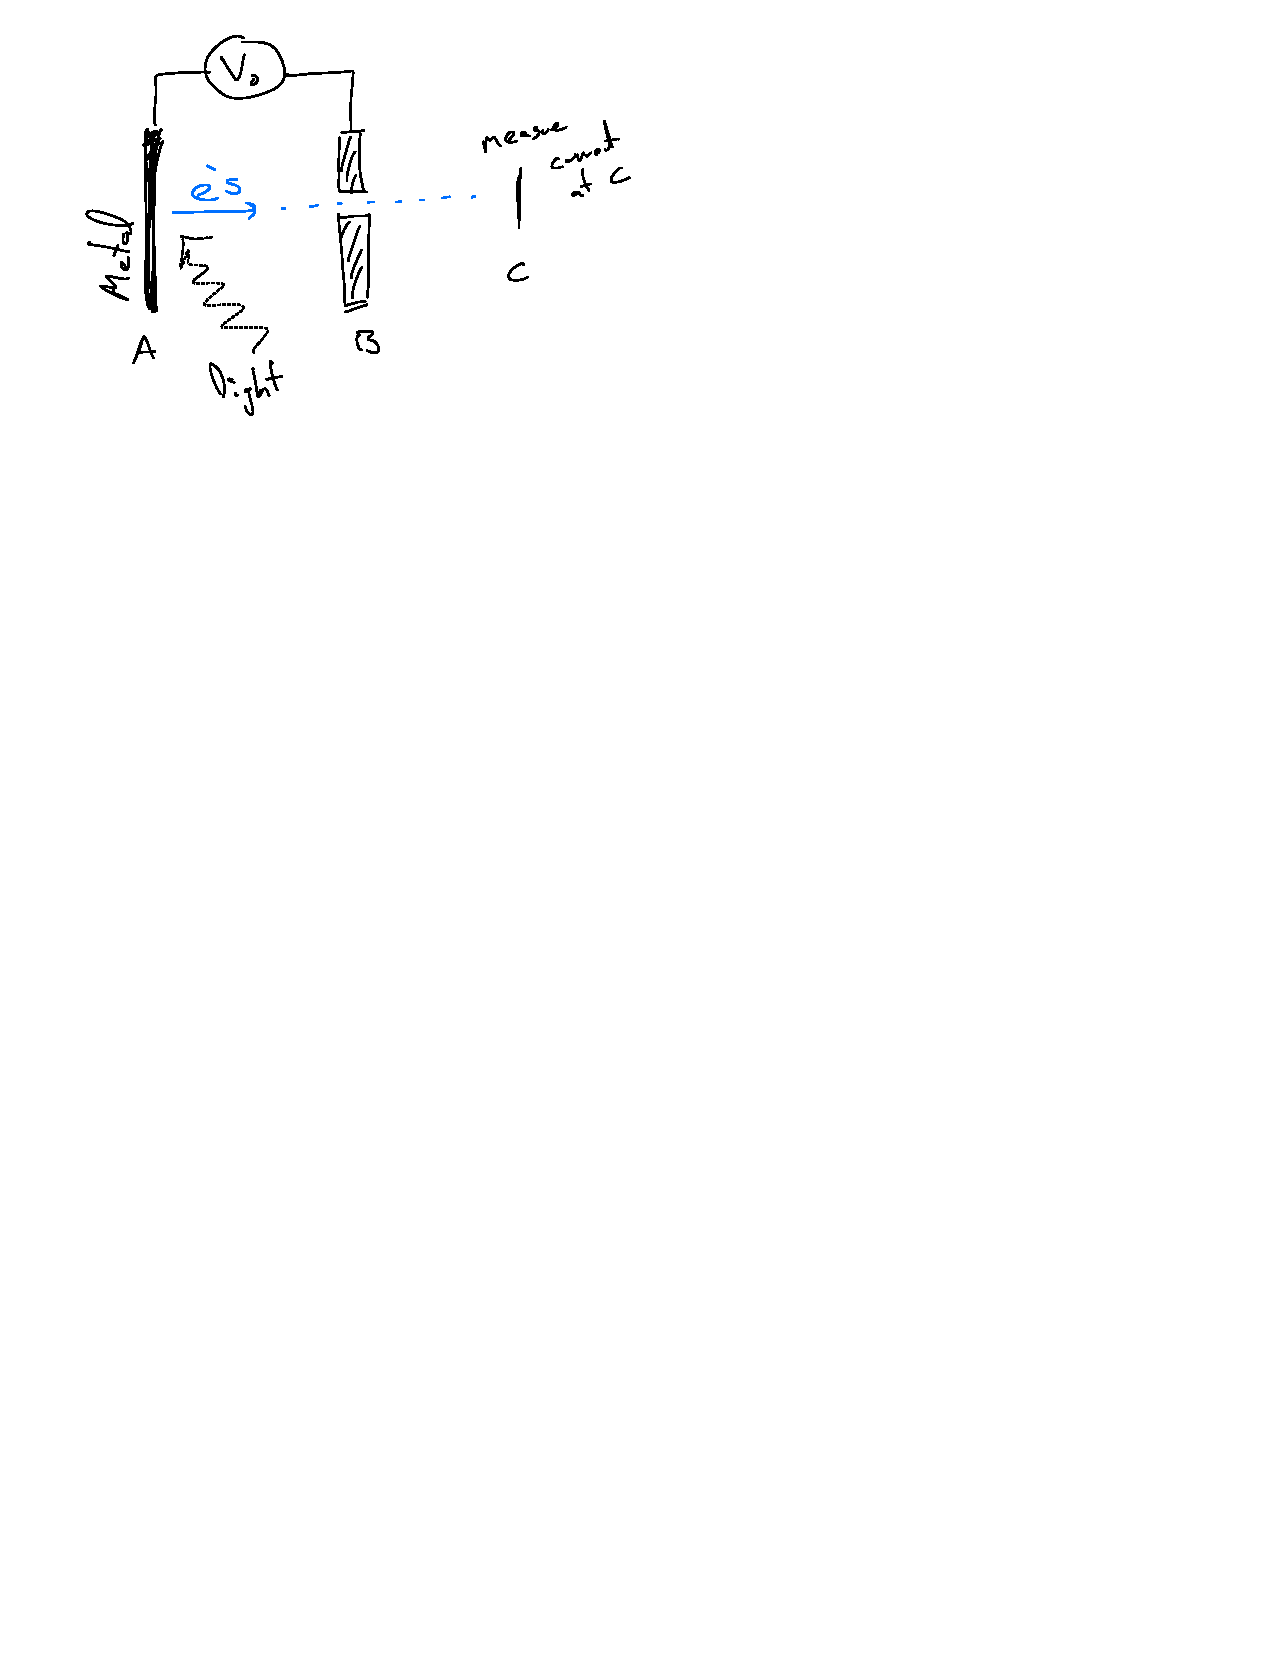
\includegraphics[width=0.5\textwidth]{./PhotoelectricExp.pdf}
\end{center}
For some voltage, referred to as the ``stopping voltage'', no current is seen.
Sketch a graph of the stopping voltage as a function of the frequency of incident light.
Assume the electrons in the metal have a binding energy of $\phi$ (i.e.: $\phi$ is the  work function of the metal).
What is the equation of the curve?


\clearpage

\textbf{12) Bohr Model} \hfill \textit{(6 points)}\\
According to the Bohr Model, how much smaller/bigger is a hydrogen atom in its first excited state compared to the ground state?

\vfill

\textbf{13) Particles As Waves } \hfill \textit{(10 points)}\\
\begin{itemize}
\item[-] Use the uncertainty principle to estimate the size (ie radius) of a hydrogen atom. \\ \textit{(Express your result in terms of $m_e$ and $\alpha$ )}
\vfill
\item[-] Use the uncertainty principle to estimate the size (ie radius) of a positronium atom. A bound state of an electron and an anti-electron (positron) \\ \textit{(Express your result in terms of $m_e$ and $\alpha$ )}
\vfill
\end{itemize}


\clearpage

\begin{minipage}{\textwidth}
\textbf{14) Quantum Mechanics} \hfill \textit{(14 points)}
\begin{itemize}
\item[-] {Consider the following wave functions $\psi_a$ and $\psi_b$:

\begin{center}
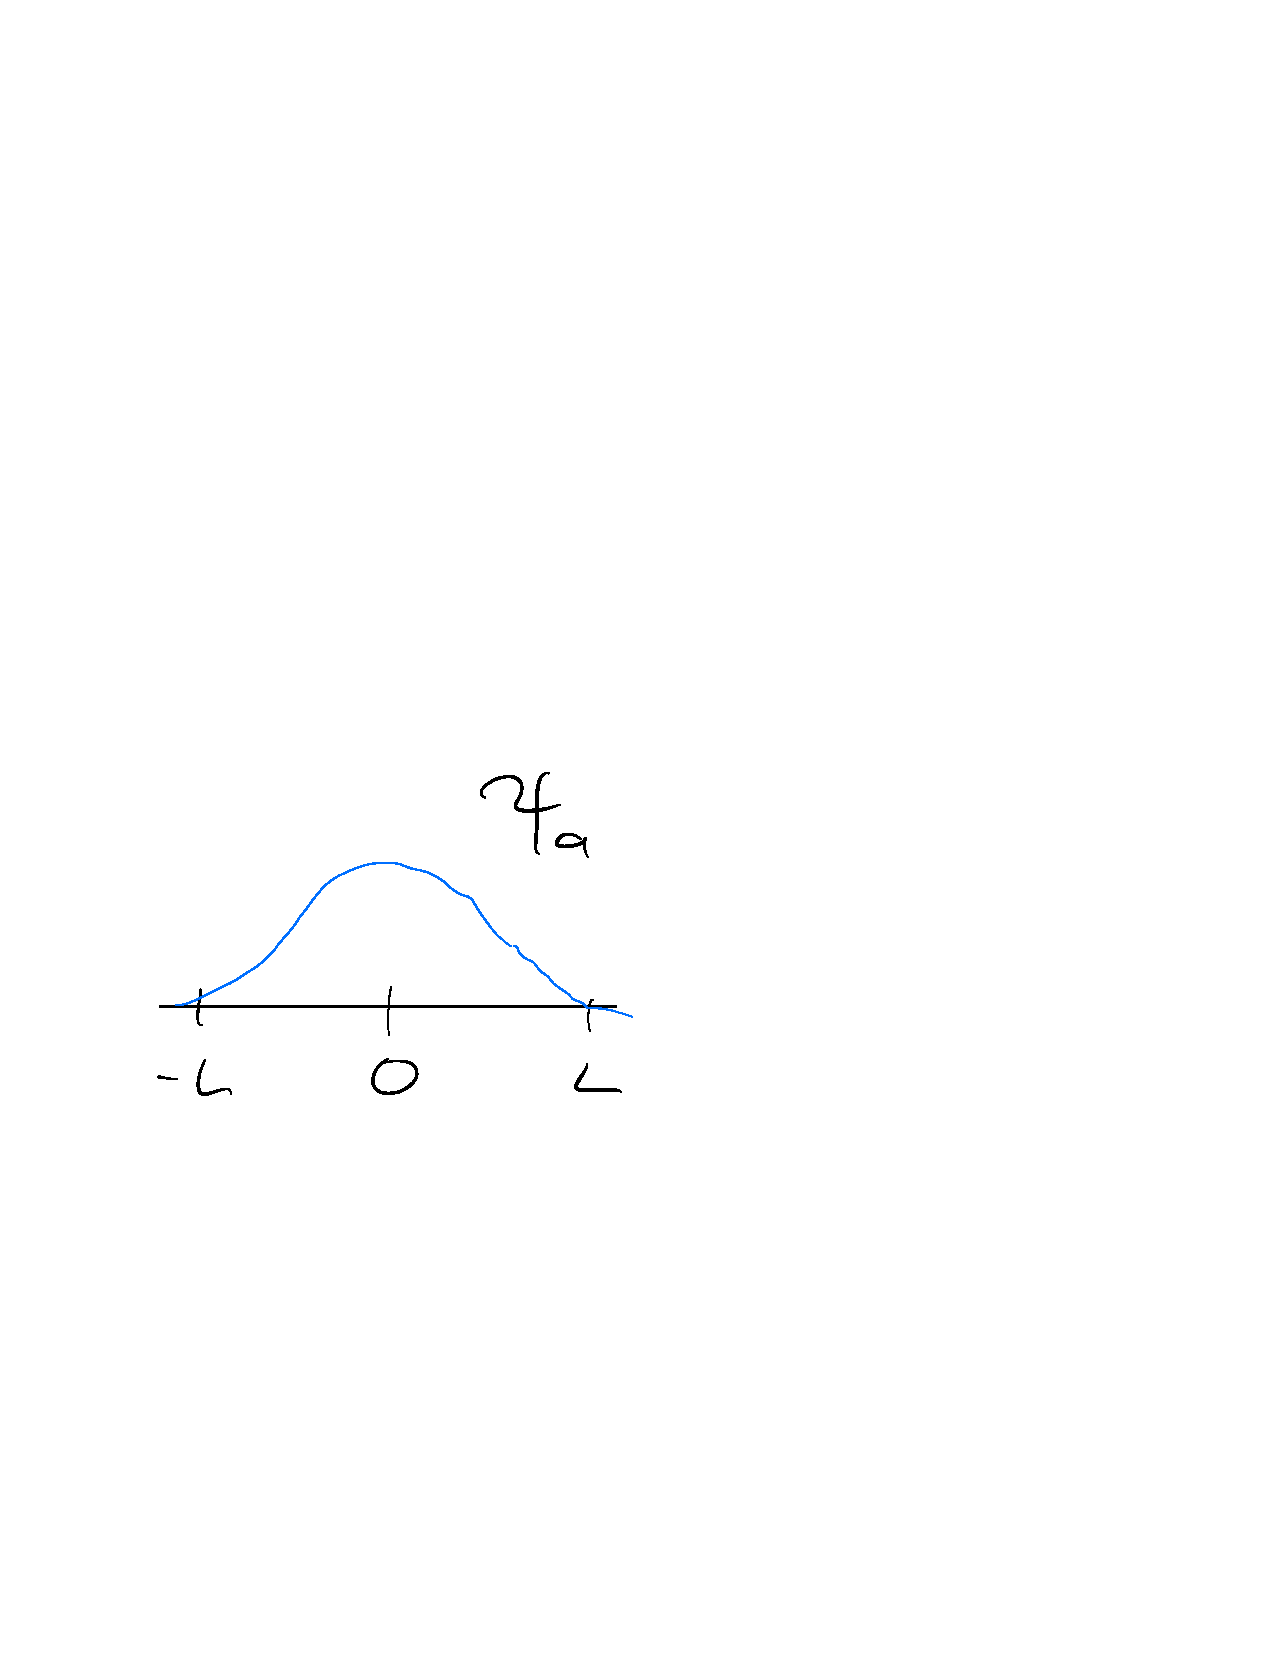
\includegraphics[width=0.3\textwidth]{./psia.pdf}
\hspace{0.3in}
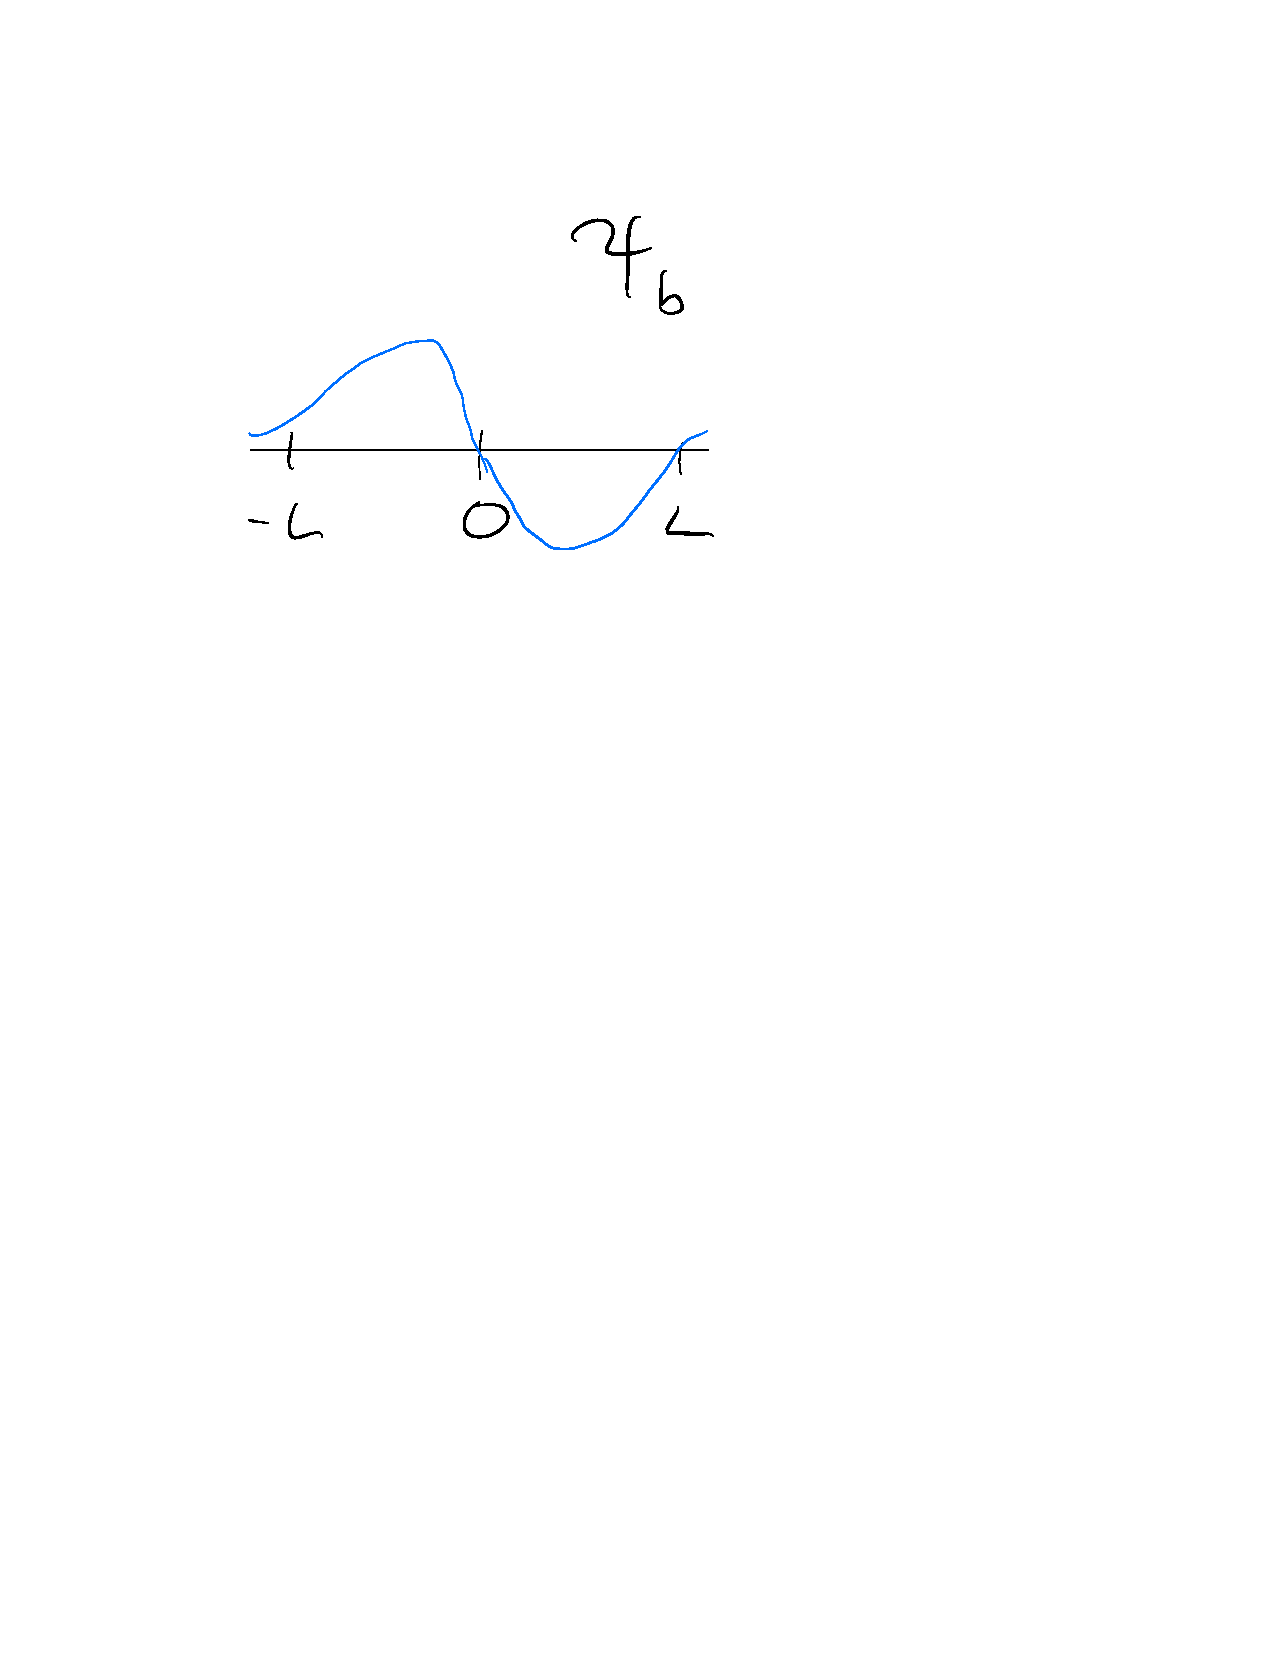
\includegraphics[width=0.3\textwidth]{./psib.pdf}
\end{center}

\begin{itemize}
\item[(a)]
Which wave function has the larger expectation value for $<x^2>$ ?
Which wave function has the larger expectation value for $<p^2>$ ? Justify your answer.
\vspace*{1.5in}
\item[(b)]
Suppose you start with a particle with wave-function $\psi_b$ and repeatedly measured it's position,
sketch the expected distribution of position measurements. 
\vspace*{1.5in}
\item[(c)]
Suppose you start with an ensemble of different particles, each with wave-function $\psi_b$, and measure each of their positions,
sketch the expected distribution of position measurements. 
\vspace*{1.5in}
\end{itemize}
}
\end{itemize}
\end{minipage}

\vspace{0.25in}

\begin{minipage}{\textwidth}
\textbf{15) More Quantum Mechanics} \hfill \textit{(12 points)}
\begin{itemize}
\item[-] What are ``Stationary States''? What is stationary about them ?
\vspace*{1.in}
\item[-] Describe what we mean by the normalization condition? 
\vspace*{1.in}
\item[-] Why is it important to have wave functions that are normalized?
\vspace*{1.in}
\end{itemize}
\end{minipage}


\begin{minipage}{\textwidth}
\textbf{16) Finite Square Well. } \hfill \textit{(10 points)}
\begin{itemize}
\item[a] Sketch the ground state and first excited state wave functions for the finite square well of length L.
\vspace*{1.5in}
\item[b] What are two differences between the solutions of the finite square well and infinite square well assuming the same length (L).
\end{itemize}
\end{minipage}


\clearpage

\textbf{17) Indistinguishable Particles. } \hfill \textit{(15 points)}
\begin{itemize}
\item[-]{ %3
Two electrons are in an infinite square well of width L.
What is the minimum total energy that the system can have? 
}
\vspace*{2.5in}
\item[-]{ %3 
What is the minimum total energy that three electrons in the system can have? 
}
\vspace*{2.5in}
\item[-]{ %3
How would the answers to a) and b) change if electrons where bosons ?
}
\end{itemize}

\clearpage

\begin{minipage}{\textwidth}
\textbf{18) Molecules. }\hfill \textit{(12 points)}
\begin{itemize}
\item[-] Use the infinite well as a model to analyze:  % 5
\begin{equation}
He + He \rightarrow He_2 
\end{equation}
Treat $He$ as infinite well of length L and $He_2$ and an infinite well of length 3/2 L.
Do you expect $He_2$ to be stable ? Why, why not? (Use the results of the infinite well model to argue your case).
\end{itemize}
\end{minipage}

\begin{minipage}{\textwidth}
\textbf{19) Infinite Square Well. }  \hfill \textit{(10 points)}
\begin{itemize}
\item[-] Write down the time-independent Schrodinger equation for the infinite square well potential in 2D. %2
\vspace*{2.5in}
\item[-] How many quantum numbers are there ?  %2
\vspace*{2.5in}
\item[-] How does the energy depend on the quantum number(s) ? %2
\vspace*{2.5in}
\end{itemize}
\end{minipage}

\clearpage

\textbf{20) Double Slit experiments. }  \hfill \textit{(10 points)}
\begin{itemize}
\item[a)]
Qualitatively discuss/sketch the observed distribution of the electrons passing through the double slit experiment.
How is this distribution accounted for in Quantum Mechanics ?
\item[b)]\vspace{3in}
Qualitatively discuss/sketch the observed distribution of the electrons passing through the double slit experiment when the path of the electron is measured.
How is this distribution accounted for in Quantum Mechanics ?
\end{itemize}



} % Begning Large
\end{document}
